% ==============================================================================
% ŠABLONA MATURITNÍ PRÁCE S OBHAJOBOU (MPsO)
% Střední průmyslová škola a Gymnázium Na Třebešíně
% ==============================================================================
% Architektura šablony přesně odpovídá dokončeným maturitním pracím na škole
% (včetně rozdělení na Úvod s cíli, Teoretickou část, Praktickou část a Závěr)
% a normě 2026-27_SPSG_sablona_MPsO.dotx 1:1.
% ==============================================================================

\documentclass[12pt, a4paper, oneside]{article}

% ------------------------------------------------------------------------------
% 1. ÚDAJE O PRÁCI (VYPLŇTE ZDE — PROPÍŠE SE AUTOMATICKY DO CELÉHO DOKUMENTU)
% ------------------------------------------------------------------------------
\newcommand{\NazevPrace}{Interaktivní digitální poznámkový blok s~integrovaným AI asistentem pro výuku}
\newcommand{\NazevPraceVelkymi}{INTERAKTIVNÍ DIGITÁLNÍ POZNÁMKOVÝ BLOK S~INTEGROVANÝM AI ASISTENTEM PRO VÝUKU}
\newcommand{\Autor}{Kostiantyn Kudinov}
\newcommand{\Vedouci}{Mgr. Jan Souhrada}
\newcommand{\VedouciDativ}{Mgr.~Janu Souhradovi}
\newcommand{\Trida}{4.G}
\newcommand{\SkolniRok}{2026 / 2027}

% ------------------------------------------------------------------------------
% 2. KÓDOVÁNÍ, JAZYK A PÍSMA (Times New Roman 12pt + Arial pro nadpisy)
% ------------------------------------------------------------------------------
\usepackage[utf8]{inputenc}
\usepackage[T1]{fontenc}
\usepackage[czech]{babel}

% Patkové písmo pro běžný text (Times New Roman / TeX Gyre Termes)
\usepackage{tgtermes}
% Bezpatkové písmo pro nadpisy a titulní stranu (Arial / Helvetica / TeX Gyre Heros)
\usepackage{tgheros}
% Neproporcionální písmo pro kód (TeX Gyre Cursor)
\usepackage{tgcursor}

% Mikrotypografie (optické vyrovnání okrajů)
\usepackage{microtype}

% ------------------------------------------------------------------------------
% 3. OKRAJE STRÁNKY A ŘÁDKOVÁNÍ (přesně dle .dotx: okraje 2,5 cm, řádkování 1,5)
% ------------------------------------------------------------------------------
\usepackage[
    a4paper,
    top=2.5cm,
    bottom=2.5cm,
    left=2.5cm,
    right=2.5cm,
    footskip=1.25cm
]{geometry}

% Řádkování 1,5 (odpovídá w:line="360" ve Wordu)
\usepackage{setspace}
\onehalfspacing

% Odstavce bez odsazení prvního řádku, mezera 6pt za odstavcem (w:after="120")
\setlength{\parindent}{0pt}
\setlength{\parskip}{6pt}

% ------------------------------------------------------------------------------
% 4. ZÁHLAVÍ, ZÁPATÍ A ČÍSLOVÁNÍ STRAN (formát "- 5 -" od 5. strany)
% ------------------------------------------------------------------------------
\usepackage{fancyhdr}

% Formát čísla stránky s pomlčkami (odpovídá w:fmt="numberInDash" v šabloně .dotx)
\renewcommand{\thepage}{- \arabic{page} -}

\pagestyle{fancy}
\fancyhf{}
\renewcommand{\headrulewidth}{0pt}
\renewcommand{\footrulewidth}{0pt}
\fancyfoot[C]{\normalfont\fontsize{12pt}{14pt}\selectfont \thepage}

% ------------------------------------------------------------------------------
% 5. FORMÁTOVÁNÍ NADPISŮ (přesně podle stylů Nadpis 1–5 v šabloně .dotx)
% ------------------------------------------------------------------------------
\usepackage{titlesec}
\usepackage{etoolbox}

% Číslování nadpisů až do 4. úrovně (2.1.1.1)
\setcounter{secnumdepth}{4}
% Zobrazení v obsahu do 3. úrovně (2.1.1)
\setcounter{tocdepth}{3}

% Každá hlavní kapitola (\section) začíná na nové stránce
\preto{\section}{\clearpage}

% Nadpis 1 (\section): 16pt, bezpatkové (Arial), tučné, mezera za 12pt
\titleformat{\section}
    {\normalfont\fontsize{16pt}{20pt}\selectfont\sffamily\bfseries}
    {\thesection}{0.75em}{}
\titlespacing*{\section}{0pt}{0pt}{12pt}

% Nadpis 2 (\subsection): 14pt, bezpatkové (Arial), tučné + kurzíva, před 12pt, za 6pt
\titleformat{\subsection}
    {\normalfont\fontsize{14pt}{18pt}\selectfont\sffamily\bfseries\itshape}
    {\thesubsection}{0.75em}{}
\titlespacing*{\subsection}{0pt}{12pt}{6pt}

% Nadpis 3 (\subsubsection): 12pt, bezpatkové (Arial), tučné, před 6pt, za 6pt
\titleformat{\subsubsection}
    {\normalfont\fontsize{12pt}{15pt}\selectfont\sffamily\bfseries}
    {\thesubsubsection}{0.75em}{}
\titlespacing*{\subsubsection}{0pt}{6pt}{6pt}

% Nadpis 4 (\paragraph): 13pt, bezpatkové (Arial), tučné, samostatný řádek
\titleformat{\paragraph}[hang]
    {\normalfont\fontsize{13pt}{16pt}\selectfont\sffamily\bfseries}
    {\theparagraph}{0.75em}{}
\titlespacing*{\paragraph}{0pt}{6pt}{6pt}

% Nadpis 5 / Podnadpis (\subparagraph): 12pt, bezpatkové (Arial), tučné, nečíslovaný
\titleformat{\subparagraph}[hang]
    {\normalfont\fontsize{12pt}{15pt}\selectfont\sffamily\bfseries}
    {}{0pt}{}
\titlespacing*{\subparagraph}{0pt}{6pt}{4pt}

% Nadpis mimo obsah (Čestné prohlášení, Poděkování, Abstrakt, Obsah...)
\newcommand{\nadpismimoobsah}[1]{%
    \vspace{6pt}%
    {\normalfont\fontsize{14pt}{18pt}\selectfont\sffamily\bfseries #1\par}%
    \vspace{2pt}%
}

% ------------------------------------------------------------------------------
% 6. OBSAH, SEZNAM OBRÁZKŮ A SEZNAM TABULEK
% ------------------------------------------------------------------------------
\makeatletter
\renewcommand{\@pnumwidth}{3.2em}
\renewcommand{\@tocrmarg}{4.0em}

% Tečkované vodící linky v Obsahu pro \section (stejně jako u podkapitol)
\renewcommand*\l@section[2]{%
  \ifnum \c@tocdepth >\z@
    \addpenalty\@secpenalty
    \addvspace{4pt \@plus\p@}%
    \setlength\@tempdima{1.8em}%
    \begingroup
      \parindent \z@ \rightskip \@pnumwidth
      \parfillskip -\@pnumwidth
      \leavevmode
      \advance\leftskip\@tempdima
      \hskip -\leftskip
      #1\nobreak\leaders\hbox{$\m@th\mkern \@dotsep mu\hbox{.}\mkern \@dotsep mu$}\hfill\nobreak\hb@xt@\@pnumwidth{\hss #2}\par
    \endgroup
  \fi}

% Položky v Seznamu obrázků ("Obrázek 1: Název ...... - 3 -")
\renewcommand*\l@figure[2]{%
  \@dottedtocline{1}{0pt}{5.5em}{Obrázek~#1}{#2}}

% Položky v Seznamu tabulek ("Tabulka 1: Název ...... - 3 -")
\renewcommand*\l@table[2]{%
  \@dottedtocline{1}{0pt}{5.5em}{Tabulka~#1}{#2}}
\makeatother

% ------------------------------------------------------------------------------
% 7. BALÍČKY PRO GRAFIKU, TABULKY, MATEMATIKU, KÓD A ODKAZY
% ------------------------------------------------------------------------------
\usepackage{graphicx}
\usepackage{float}
\usepackage{url}
\usepackage{booktabs}
\usepackage{array}
\usepackage{tabularx}
\usepackage{amsmath}
\usepackage{amssymb}
\usepackage{enumitem}
\usepackage{xcolor}
\usepackage{listings}

% Popisky obrázků a tabulek dle .dotx: kurzíva, zarovnáno na střed
\usepackage[
    font={it},
    labelfont={it},
    labelsep=colon,
    justification=centering
]{caption}

\addto\captionsczech{%
    \renewcommand{\figurename}{Obr.}%
    \renewcommand{\tablename}{Tab.}%
}

% Konfigurace pro výpisy zdrojového kódu (listings)
\definecolor{codebg}{rgb}{0.97, 0.97, 0.97}
\definecolor{codeborder}{rgb}{0.85, 0.85, 0.85}
\definecolor{codecomment}{rgb}{0.40, 0.40, 0.40}
\definecolor{codekeyword}{rgb}{0.10, 0.20, 0.70}
\definecolor{codestring}{rgb}{0.15, 0.50, 0.15}

\lstset{
    backgroundcolor=\color{codebg},
    frame=single,
    rulecolor=\color{codeborder},
    basicstyle=\ttfamily\fontsize{9.5pt}{12pt}\selectfont,
    keywordstyle=\color{codekeyword}\bfseries,
    commentstyle=\color{codecomment}\itshape,
    stringstyle=\color{codestring},
    numbers=left,
    numberstyle=\tiny\color{codecomment},
    numbersep=8pt,
    breaklines=true,
    breakatwhitespace=true,
    showstringspaces=false,
    tabsize=2,
    captionpos=b,
    keepspaces=true
}

% Klikací hypertextové odkazy v PDF (bez rušivých rámečků)
\usepackage[hypertexnames=false, hidelinks, unicode]{hyperref}


% ==============================================================================
% DOKUMENT
% ==============================================================================
\begin{document}

% Strany 1–4 nemají zobrazené číslo strany v zápatí
\pagestyle{empty}

% ------------------------------------------------------------------------------
% STRANA 1: TITULNÍ LIST
% ------------------------------------------------------------------------------
\begin{center}
    {\sffamily\fontsize{12pt}{15pt}\selectfont Střední průmyslová škola a~Gymnázium Na Třebešíně\par}
    \vspace{6pt}
    {\sffamily\bfseries\fontsize{16pt}{20pt}\selectfont MATURITNÍ PRÁCE S~OBHAJOBOU\par}

    \vspace{1.2cm}
    
\includegraphics[width=5.6cm]{obrazky/logo_skoly.png}

    \vspace{2.2cm}
    {\sffamily\bfseries\fontsize{16pt}{22pt}\selectfont \NazevPraceVelkymi\par}
\end{center}

\vfill

{\sffamily\fontsize{10pt}{14pt}\selectfont
\begin{tabular}{@{}p{3.5cm}l@{}}
    Vypracoval: & \Autor \\[6pt]
    Vedoucí:    & \Vedouci \\[6pt]
    Třída:      & \Trida \\[6pt]
    Školní rok: & \SkolniRok \\
\end{tabular}
}

\vspace{0.5cm}
\clearpage

% ------------------------------------------------------------------------------
% STRANA 2: ZADÁNÍ (NASKENOVANÝ DOKUMENT)
% ------------------------------------------------------------------------------
\noindent
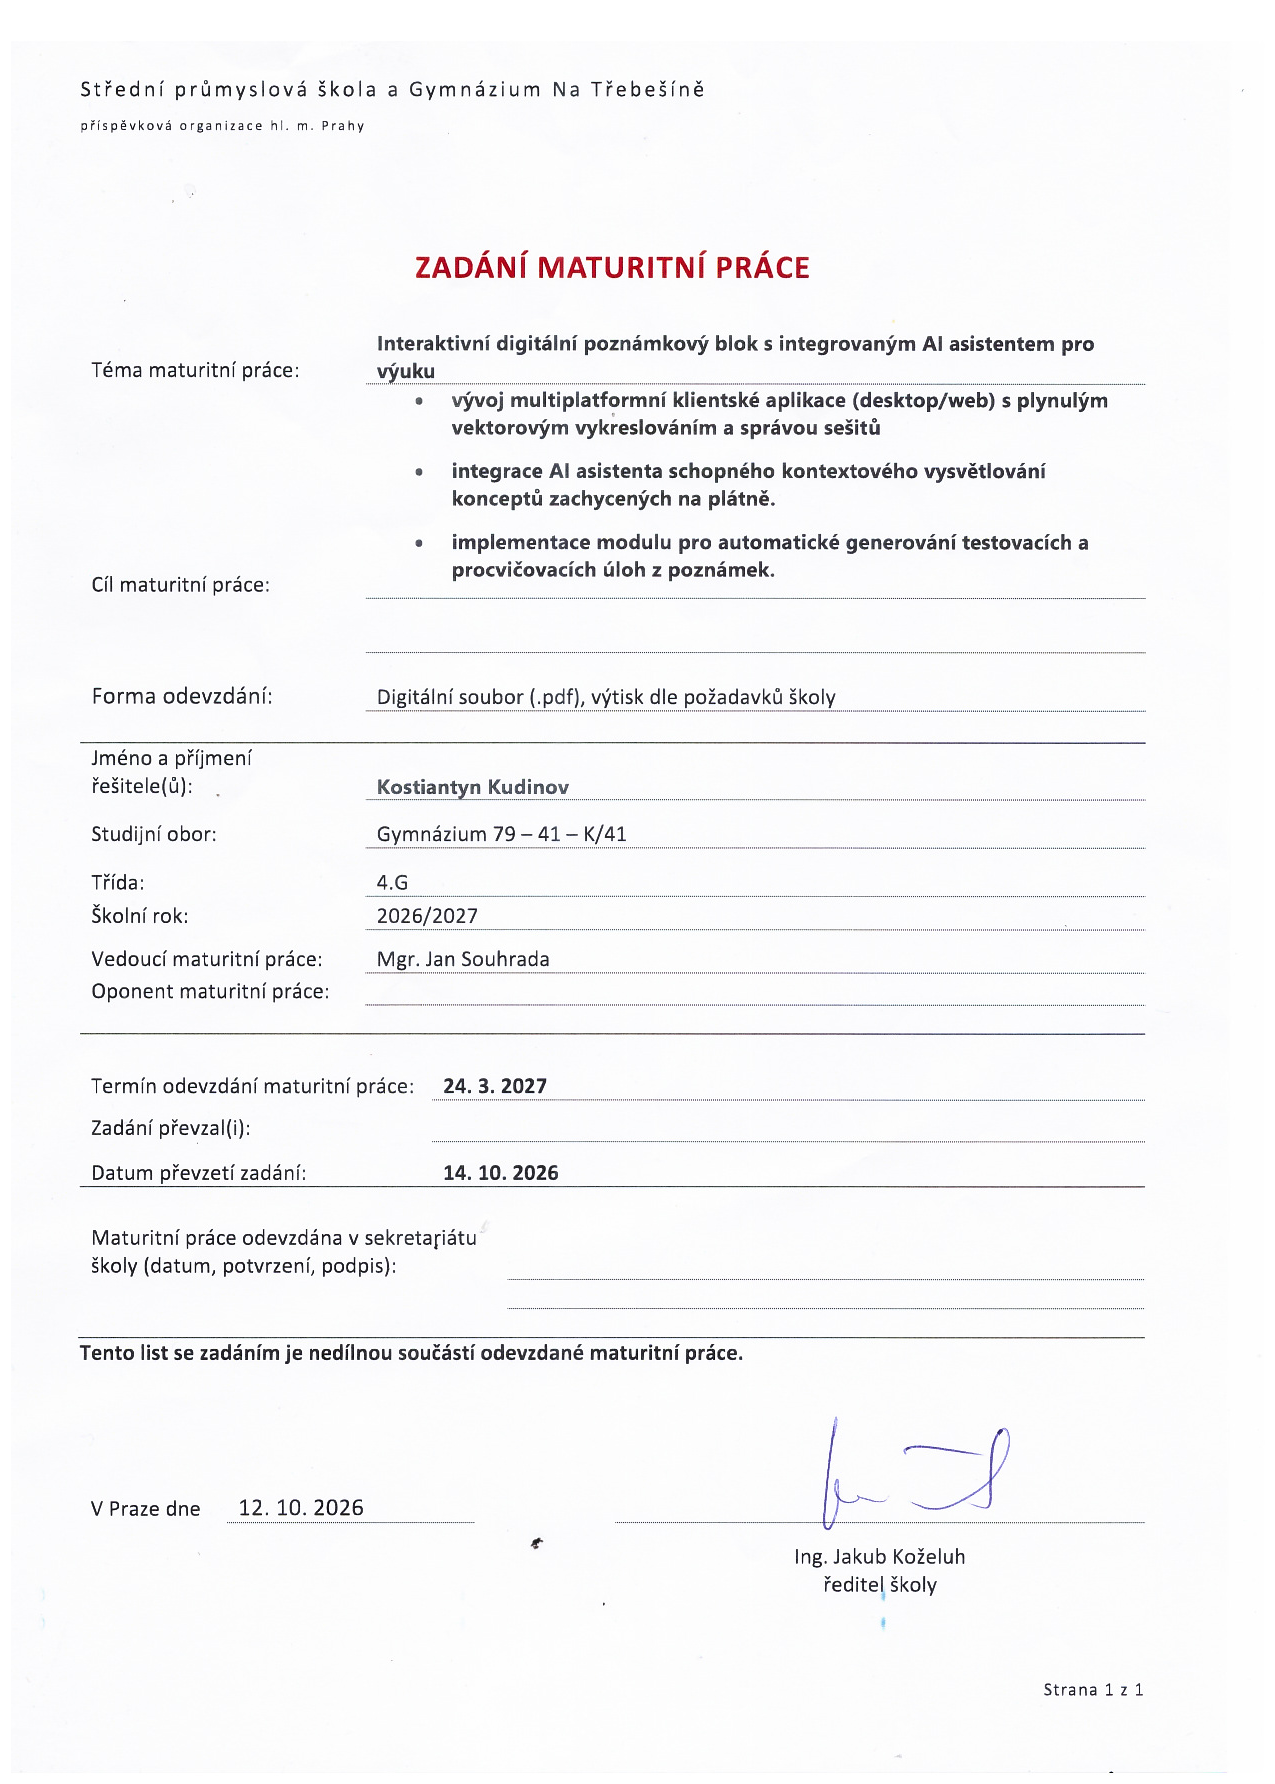
\includegraphics[width=\textwidth]{obrazky/zadani.png}

\clearpage

% ------------------------------------------------------------------------------
% STRANA 3: ČESTNÉ PROHLÁŠENÍ
% ------------------------------------------------------------------------------
\vspace*{7.5cm}

\nadpismimoobsah{Čestné prohlášení}

Prohlašuji, že jsem maturitní práci na téma \textbf{\NazevPrace} vypracoval(a) samostatně s~využitím odborné literatury a~pramenů uvedených v~přiloženém seznamu využitých zdrojů.

\vspace{1.2cm}
V~Praze dne: \makebox[4cm]{\dotfill}

\vspace{1.8cm}
\makebox[6cm]{\dotfill} \\
\textit{Podpis autora}

\clearpage

% ------------------------------------------------------------------------------
% STRANA 4: PODĚKOVÁNÍ
% ------------------------------------------------------------------------------
\vspace*{6.5cm}

\nadpismimoobsah{Poděkování}

Děkuji tímto vedoucímu maturitní práce panu \textbf{\VedouciDativ} za odborné vedení, cenné připomínky, věcné rady a~čas věnovaný konzultacím při zpracování této práce.

\clearpage

% ==============================================================================
% OD STRANY 5: ČÍSLOVÁNÍ STRAN DOLE UPROSTŘED ("- 5 -")
% ==============================================================================
\pagestyle{fancy}
\setcounter{page}{5}

% ------------------------------------------------------------------------------
% STRANA 5: ANOTAČNÍ LIST (ČESKY)
% ------------------------------------------------------------------------------
\nadpismimoobsah{Název práce:}
\NazevPrace

\nadpismimoobsah{Autor:}
\Autor

\nadpismimoobsah{Vedoucí práce:}
\Vedouci

\nadpismimoobsah{Abstrakt}
Cílem této maturitní práce je navrhnout, implementovat a~otestovat odlehčený, multiplatformní digitální poznámkový blok a~virtuální tabuli s~integrovaným asistentem na bázi umělé inteligence pro podporu výuky a~samostatného studia. Aplikace kombinuje výhody neomezené plochy (ZUI) pro volné myšlenkové mapy se stránkovaným sešitem formátu A4 a~možností importu i~anotování dokumentů PDF. Klientská vrstva je postavena na frameworku Tauri~v2, jazyce Rust a~knihovně React s~využitím HTML5 Canvasu pro plynulé vektorové vykreslování s~minimální latencí. Na rozdíl od běžných komerčních řešení je aplikace navržena podle principů Local-First – veškeré poznámky jsou ukládány primárně lokálně na disk v~přenosném formátu bez nutnosti zakládání uživatelského účtu. Součástí projektu je také integrovaný multimodální AI asistent pro kontextové vysvětlování ručně psané látky a~tvorbu procvičovacích úloh.

\nadpismimoobsah{Klíčová slova}
digitální poznámkový blok, virtuální tabule, Tauri v2, Rust, React, TypeScript, HTML5 Canvas, Local-First, offline-first, anotace PDF, umělá inteligence, multimodální AI

\clearpage

% ------------------------------------------------------------------------------
% STRANA 6: ANOTAČNÍ LIST (ANGLICKY — SUMMARY)
% ------------------------------------------------------------------------------
\nadpismimoobsah{Summary}
The objective of this graduation thesis is to design, implement, and evaluate a~lightweight, cross-platform digital notebook and virtual whiteboard application with an integrated artificial intelligence assistant for educational workflows and self-directed study. The system merges the affordances of an infinite zoomable canvas (ZUI) for mind mapping with a~structured ISO~216 A4 paginated notebook capable of importing and annotating PDF documents. Engineered atop Tauri~v2, Rust, and React, the client utilizes an immediate-mode HTML5 Canvas rendering architecture to ensure low-latency pen input and smooth 60~FPS performance. In contrast to conventional cloud-dependent solutions, the application follows Local-First design principles, storing notebooks directly on the user's local disk in a~portable format without requiring an account. Furthermore, an interactive multimodal AI tutor is integrated to provide contextual explanations of handwritten calculations and generate automated practice questions.

\nadpismimoobsah{Keywords}
digital notebook, virtual whiteboard, Tauri v2, Rust, React, TypeScript, HTML5 Canvas, Local-First, offline-first, PDF annotation, artificial intelligence, multimodal AI

\clearpage

% ------------------------------------------------------------------------------
% STRANA 7: OBSAH
% ------------------------------------------------------------------------------
\nadpismimoobsah{Obsah}
\makeatletter
\@starttoc{toc}
\makeatother

\clearpage

% ==============================================================================
% 1 ÚVOD
% ==============================================================================
\section{Úvod}
\label{sec:uvod}

Při studiu technických oborů a~programování běžné textové procesory jako Microsoft Word nebo Google Docs nestačí. Psaní matematických vzorců, kreslení schémat a~náčrty algoritmů jsou v~nich zdlouhavé a~nepraktické. Mnohem přirozenější je psát a~kreslit volnou rukou na digitálním plátně nebo vpisovat poznámky přímo do přednáškových materiálů ve formátu PDF.

Dostupné aplikace pro digitální poznámky však mají své slabiny. Většina nástrojů nenabízí verzi pro Linux a~zbytek bývá často postaven na frameworku Electron, což znamená vysokou spotřebu paměti RAM a~znatelnou odezvu při kreslení perem kvůli vestavěnému jádru Chromium. Komerční řešení navíc často vyžadují vytvoření online účtu a~ukládání veškerých dat do cloudu. Uživatel tak nemá své soubory plně pod kontrolou a~bez internetového připojení se k~nim nedostane.

Prakticky jedinou rozšířenou aplikací, která se těmto problémům vyhýbá a~funguje nativně na Linuxu, je Xournal++. V~některých ohledech však zaostává za moderními digitálními sešity – chybí jí režim nekonečného plátna, neumožňuje spuštění v~prohlížeči a~její tradiční uživatelské rozhraní schovává řadu funkcí do větvených nabídek či drobných tlačítek, což při ovládání perem a~dotykem působí nepohodlně.

Tato práce se zabývá vývojem lehkého digitálního poznámkového bloku, který spojuje přívětivé rozhraní moderních aplikací s~rychlou a~efektivní Local-First filozofií programu Xournal++. Aplikace funguje jako desktopový program pro Linux a~Windows, lze ji však spustit i~ve webovém prohlížeči či na zařízeních se systémem Android. Projekt kombinuje nekonečnou plochu pro myšlenkové mapy se stránkovaným sešitem formátu A4. Poznámky se ukládají primárně lokálně na disk v~přenosném formátu. Součástí je také jednoduchý AI asistent, který pomáhá s~vysvětlením probírané látky nebo tvorbou procvičovacích otázek přímo z~obsahu sešitu.

% ------------------------------------------------------------------------------
% 1.1 CÍLE PRÁCE
% ------------------------------------------------------------------------------
\subsection{Cíle práce}
\label{sec:cile_prace}

\begin{enumerate}
    \item Naprogramování multiplatformní aplikace digitálního poznámkového bloku pomocí frameworku Tauri~v2, jazyka Rust a~knihovny React.
    \item Vytvoření interaktivního plátna s~volbou mezi nekonečnou plochou a~stránkovaným sešitem formátu A4, včetně možnosti importu a~anotování dokumentů PDF.
    \item Lokální ukládání sešitů na disk ve vlastním přenosném formátu s~možností synchronizace do cloudového úložiště.
    \item Integrace interaktivního AI asistenta pro generování vysvětlení a~procvičovacích otázek na základě kontextu ze sešitu.
\end{enumerate}


% ==============================================================================
% 2 TEORETICKÁ ČÁST
% ==============================================================================
\section{Teoretická část}
\label{sec:teoreticka_cast}

Teoretická část práce se věnuje rozboru klíčových konceptů, na nichž je návrh aplikace vystavěn. Zahrnuje problematiku interakce člověka s~počítačem (HCI) v~prostředí digitálních poznámek, matematické principy počítačové 2D grafiky a~souřadnicových transformací, zásady architektury Local-First a~zhodnocení použitých technologií.

% ------------------------------------------------------------------------------
% 2.1 DIGITÁLNÍ PRACOVNÍ PROSTORY A UŽIVATELSKÁ ROZHRANÍ
% ------------------------------------------------------------------------------
\subsection{Digitální pracovní prostory a uživatelská rozhraní}
\label{sec:teorie_zui}

V~oblasti softwaru pro zaznamenávání informací existují dva protichůdné přístupy k~organizaci pracovní plochy: neomezená prostorová plocha a~diskrétní stránkovaný dokument.

\subsubsection{Koncept nekonečného plátna (ZUI)}
Koncept nekonečného plátna vychází z~paradagmatu \textit{Zoomable User Interface} (ZUI), jehož teoretické základy položili Perlin a~Fox v~roce 1993 a~dále rozvinuli Bederson a~Hollan~\cite{bederson1994pad}. V~rozhraní ZUI není pracovní prostor omezen fyzickými hranicemi okna či listu papíru; scéna existuje v~souvislé dvourozměrné eukleidovské rovině $\mathbb{R}^2$. Uživatel se v~tomto prostoru pohybuje prostřednictvím dvou základních stupňů volnosti:
\begin{itemize}
    \item \textbf{Posun (Panning):} Translace virtuální kamery v~osách $x$ a~$y$, která umožňuje procházet rozsáhlé diagramy a~myšlenkové mapy.
    \item \textbf{Změna měřítka (Zooming):} Plynulá změna faktoru zvětšení, která umožňuje pracovat na různých úrovních sémantického detailu -- od globálního nadhledu nad celým projektem až po detailní mikroskopický zápis vzorců.
\end{itemize}

Výhodou ZUI je eliminace kognitivních bariér při brainstormingu, neboť uživatel není nucen předem odhadovat potřebný rozsah stránky.

\subsubsection{Stránkovaný sešit a standard ISO 216}
Zatímco ZUI exceluje při volném plánování, při systematickém studiu a~přípravě na výuku naráží na limity při exportu a~tisku. Školní materiály, testy a~pracovní listy se opírají o~mezinárodní standard ISO~216~\cite{iso216}, který definuje formátovou řadu A. Základní formát A0 má plochu přesně $1\text{ m}^2$ a~poměr stran $1 : \sqrt{2}$, což zaručuje, že při přeložení listu na polovinu zůstává poměr stran zachován (tzv. Lichtenbergův poměr). Nejrozšířenější školní formát A4 (rozměry $210 \times 297\text{ mm}$) je pro digitální poznámkový blok ideální jednotkou: poskytuje známé vizuální ohraničení, usnadňuje vkládání a~anotaci předloh v~PDF a~umožňuje přímý tisk bez nežádoucího ořezu.

% ==============================================================================
% 3 PRAKTICKÁ ČÁST
% ==============================================================================
\section{Praktická část}
\label{sec:prakticka_cast}

\textit{(Tato kapitola bude vypracována v~průběhu realizace projektu.)}


% ==============================================================================
% 4 ZÁVĚR
% ==============================================================================
\section{Závěr}
\label{sec:zaver}

\textit{(Bude doplněno po dokončení implementace a~vyhodnocení cílů.)}



% ==============================================================================
% 5 SEZNAM VYUŽITÝCH ZDROJŮ (ČSN ISO 690)
% ==============================================================================
\section{Seznam využitých zdrojů}
\label{sec:zdroje}

\begingroup
\sloppy
\renewcommand{\section}[2]{}%
\begin{thebibliography}{99}

    \bibitem{bederson1994pad}
    BEDERSON, Benjamin B. a~James D. HOLLAN. Pad++: A~Zooming Graphical Interface for Exploring Alternate Interface Physics. In: \textit{Proceedings of the 7th Annual ACM Symposium on User Interface Software and Technology (UIST '94)} [online]. New York: ACM, 1994, s.~17--26 [cit. 2026-11-04]. ISBN 0-89791-657-3. Dostupné z: \url{https://doi.org/10.1145/192426.192435}

    \bibitem{iso216}
    INTERNATIONAL ORGANIZATION FOR STANDARDIZATION. \textit{ISO 216:2007 Writing paper and certain classes of printed matter -- Trimmed sizes} [online]. Ženeva: ISO, 2007 [cit. 2026-11-04]. Dostupné z: \url{https://www.iso.org/standard/36631.html}

\end{thebibliography}
\endgroup


% ==============================================================================
% 6 PŘÍLOHY
% ==============================================================================
\clearpage
\section*{Přílohy}
\addcontentsline{toc}{section}{Přílohy}

\textit{(Přílohy budou doplněny k~odevzdání práce.)}

\end{document}
